\section{The model}
\label{sec:the-model}
In this section we will go through the model from the article \cite{self-org} 
in great detail. As mentioned earlier in section~\ref{sec:social-forces} the 
social force model is an agent based model, this means that we describe the 
system by looking at each individual object of the system. In this case each 
object in the system is subject to a series of social forces. These forces 
are not real physical forces in the sence that they follow newtons laws of 
motion but rather a measure of the agents motivation for acting in specific 
ways. However that name \emph{social forces} is not accidential, we borrow 
both notation and to some extent the interpretation from physics. In the model 
we are studying there are four different forces. They are \emph{the desired force}, 
\emph{the repulsive force from walls}, \emph{the interaction force} and \emph{the 
attractive force}. All the forces work in the horizontal plane, the vertical 
plane is not of interest. The forces are illustrated in 
figure~\ref{ForceModel}.  They will all be studied closely in turn in the 
following sections.  But before we do this we would like to comment on the 
notation of the mathematics in the model. In the original paper the radius of 
a pedestrian is given as $r_{\alpha}$ and the position is $\vec{r_{\alpha}}$. 
This can easily confuse one, since one could think that $r_{\alpha}$ is the length 
of $\vec{r_{\alpha}}$, which it is not. So for clarity we write R for radius and p for position. I.e. $\overrightarrow{p_{\alpha}}$ is the vector from a fixed point in space to the position of $\alpha$. In general, any expression that 
has $^{0}$ is a desire. 

\begin{figure}[ht]
    \centering
    {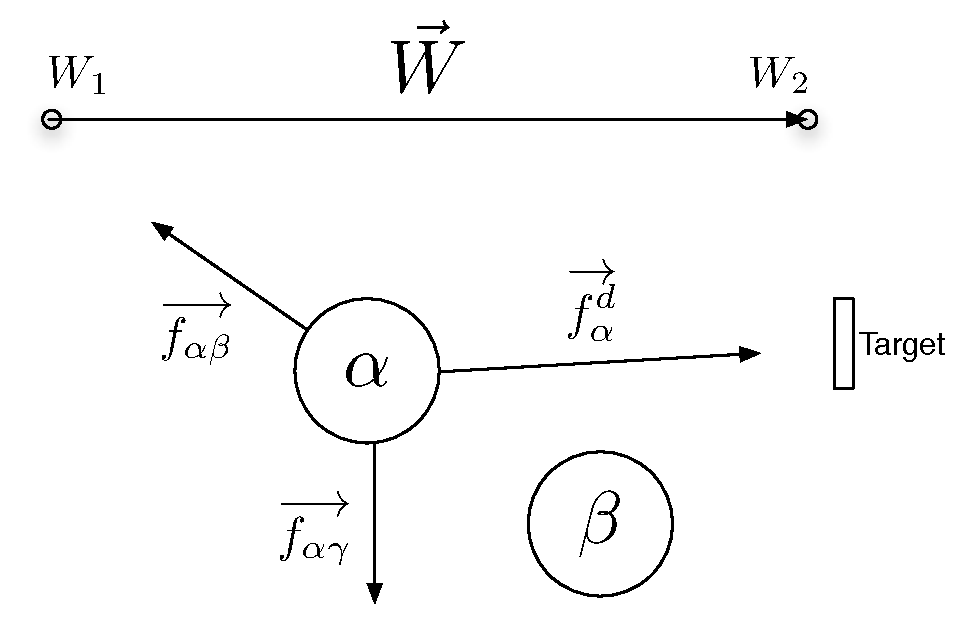
\includegraphics[scale=0.45]{Figures/ForceModel.pdf}} \caption[Notation 
    of forces acting on an agent]{Illustration of the forces acting on an 
    agent $\alpha $. $ \beta $ is another agent and the grey bar on the top 
    represents a wall. $ \overrightarrow{f_{\alpha\beta}} $ is the repulsive force from 
    agent $ \beta $, and $ \overrightarrow{f_{\alpha B}} $ is the repulsive force from 
    the wall. $ \overrightarrow{f^{0}_{\alpha}} $ is a force that represents agent $ 
    \alpha $'s desire to reach the exit.  The x and y axes are defined by the 
    Cartesian coordinate system.}
    \label{ForceModel}
\end{figure}

\subsection{The equation of motion for agent $ \alpha $:}
The purpose of the model is to describe how each agent moves so an equation of 
motion for each agent is needed. They way to get this equation of motion is 
much like one would in physics by summing up all the forces acting on the 
agent. This gives rise to an acceleration of the agent and from this one is 
able to derive the exact movement of the agent. Again it is important that 
this is a method borrowed from physics, we are not working with real physical 
forces here.

Each induvidual agent has a series of parameters describing the features of 
the agent. An agent is represented by a circle with radius $R_{\alpha}$. The 
agent has a position vector $\overrightarrow{p_{\alpha}}$ and a velocity vector $\overrightarrow{V_{\alpha}}$ at 
all times t. Furthermore each agent has a desired direction $\overrightarrow{e_{\alpha}}$ 
in which it would like to move. An illustration of the notation can be seen in 
figure \ref{fig:NotationOfAgent}.

\begin{figure}[hb]
    \centering
    {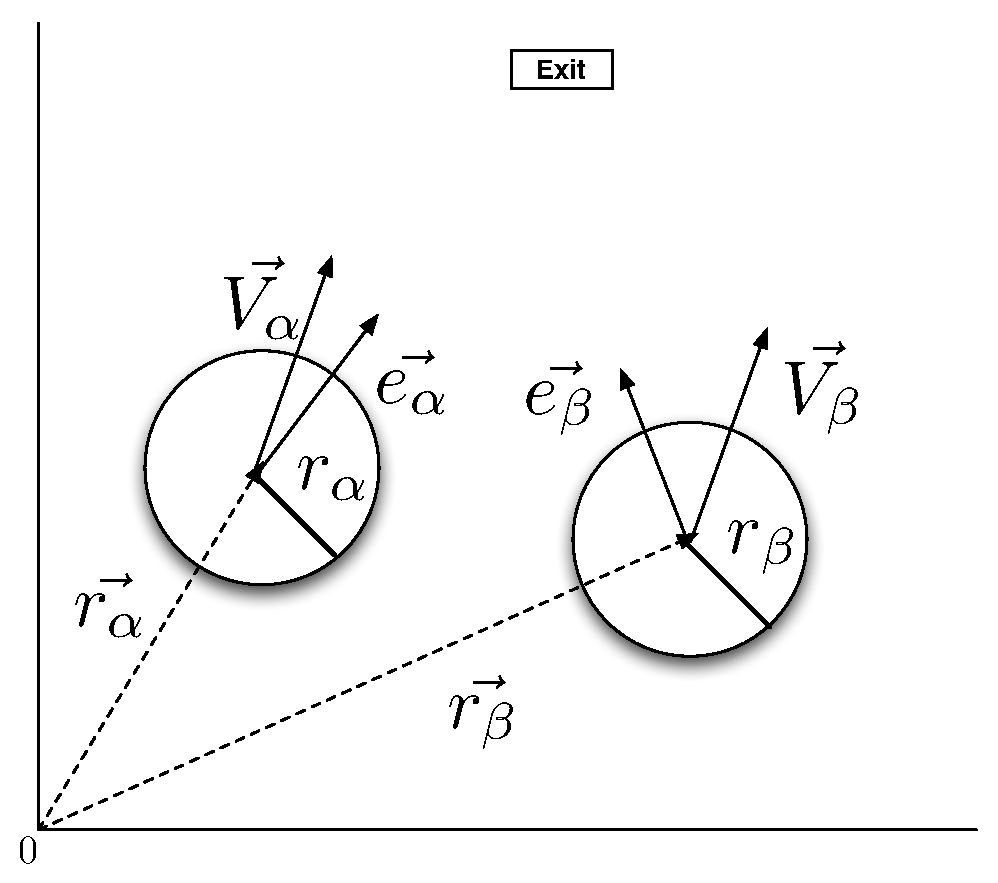
\includegraphics[scale=0.35]{Figures/NotationOfAgent.pdf}} 
    \caption[Notation of an agent]{Illustration of the visual presentation of 
    the mathematical notations for position and velocity. As for agent $ 
    \alpha $, it has position vector $ \overrightarrow{p_{\alpha}} $, velocity vector $ 
    \overrightarrow{V_{\alpha}} $, $\overrightarrow{e_{\alpha}}$ or $\overrightarrow{e_{\beta}}$ the unit 
    vector pointing to the exit and  $ R_{\alpha} $ or  $ R_{\beta} $ the 
    radius of its body.  The x and y axes are defined by the Cartesian 
    coordinate system.}
    \label{fig:NotationOfAgent}
\end{figure}

The change in position $ \overrightarrow{p_{\alpha}} $ per time of agent $\alpha$ is the 
velocity $ \overrightarrow{V_{\alpha}} $:

\begin{equation}
		\frac{d \overrightarrow{p_{\alpha}}}{dt} = \overrightarrow{V_{\alpha}} \left( t \right)
\end{equation}

The change of velocity per time is the acceleration of agent $\alpha$, which 
is due to all the forces acting on the agent is given by:

\begin{equation}
    \frac{d \overrightarrow{V_{\alpha}}}{dt} = \overrightarrow{f_{\alpha}} \left( t \right) 
\end{equation}

The summation of all the forces $\overrightarrow{f_{\alpha}}$ can be devided into four 
terms as stated in the introduction to this section.

\begin{equation}\label{model}
    \overrightarrow{f_{\alpha}} = \overrightarrow{f^{0}_{\alpha}} + \overrightarrow{f_{\alpha B}} +
    \sum_{\beta \neq \alpha} \overrightarrow{f_{\alpha \beta}} +  
    \sum_{i} \overrightarrow{f_{\alpha i}} 
\end{equation}

Here $\overrightarrow{f_{\alpha}^{0}}$ is the desired force, $\overrightarrow{f_{\alpha 
\text{B}}}$ is the repulsive force from walls. $\overrightarrow{f_{\beta\alpha}}$ 
is a repulsive force from other agents and $\overrightarrow{f_{\alpha i}}$ is a 
attractive force.

We will now move on to show the explicit expression for each force. We will go 
through them one at a time explaining their mathematical structure and their 
role in the model.

\begin{center}
\begin{tabular}{lll}
\hline
$\overrightarrow{f_{\alpha}^{0}}$ & the desired force &\\
\hline
$\overrightarrow{f_{\alpha B}}$ & the repulsive force from walls &\\
\hline
$\overrightarrow{f_{\alpha \beta}}$ & the repulsion from other agents\\
\hline
$\overrightarrow{f_{\alpha i}}$& the attractive force\\
\hline
\end{tabular}
\end{center}

\subsection{The desired force}
\label{sec:desired-force}
The first term on the right hand side of equation \eqref{model} describes the 
\emph{willingness} of agent $\alpha$'s to reach the exit. It is a velocity 
dependent force and is given by:

\begin{equation}\label{relaxtime}
	\overrightarrow{f^{0}_{\alpha}}\left( \overrightarrow{V_{\alpha}} \right) =
    \frac{1}{\tau}
    \left( V_{\alpha}^{0} \overrightarrow{e_{\alpha}} - \overrightarrow{V_{\alpha}} \right)
\end{equation}

Where $V_{\alpha}^{0}$ is the desired speed, $ \overrightarrow{e_{\alpha}} $ is the unit 
vector pointing in the desired direction of the agent which in most cases will 
be the exit, but it can in principle be anywhere.  $\overrightarrow{V_{\alpha}}$ is the 
actual velocity of the agent, and $\tau$ is the \emph{relaxation time}.

The relaxtion time determines how reactive a agent is. In principle the 
relaxation time can vary for each agent but from the article \cite{self-org} 
we get that $ \tau_{\alpha}\approx 1s $, which means that it takes the agent 
one second to change its velocity. $V_{\alpha}^{0} \overrightarrow{e_{\alpha}}$ is the desired 
velocity of the agent. The desired speed can vary over time and is given by:

\begin{equation}\label{v0eta}
    V_{\alpha}^{0}\left( t \right) = \left[ 1 - \eta_{\alpha} \left( t \right) \right] 
    V_{\alpha}^{0} \left( 0 \right) +
    \eta_{\alpha} \left( t \right)V_{\alpha}^{\text{max}}
\end{equation}
%TODO: write that V_a^0(0) < V_a^0(t) < V_a^max
where $V_{\alpha}^{0} \left( 0 \right)$ is the desired speed at $ t=0 $, and 
$V_{\alpha}^{\text{max}}$ is the maximum desired speed of agent $\alpha$. The 
maximum desired speed is the speed that agent $\alpha$ will try to get if it 
is allowed by the environment and other agents. It is not a physical limit to 
how fast the agent can move but rather a parameter that determines the speed 
that the agent is comfortable walking with. 

$\eta_{\alpha} \left( t \right)$ is called the impatience or nervousness of 
the agent and is given by:

\begin{equation}\label{eta}
	\eta_{\alpha} \left( t \right) =
    1 - \frac{\overline{V}_{\alpha} \left( t \right)}
             {V_{\alpha}^{0} \left( 0 \right)}
\end{equation}

where $\overline{V}_{\alpha}\left( t \right)$ is the average speed in the 
desired direction.Excately how one measures the average speed in the desired 
direction is not properly explained in the article. We define it to be the 
projection of the position vector $ \overrightarrow{p_{\alpha}} $ onto the desired direction 
of motion $e_{\alpha}$ devided by the time that the simulation has run. A 
illustration of this can be seen i figure \ref{impatience}. The mathematical 
expression becomes:

\begin{figure}[ht]
    \centering
    {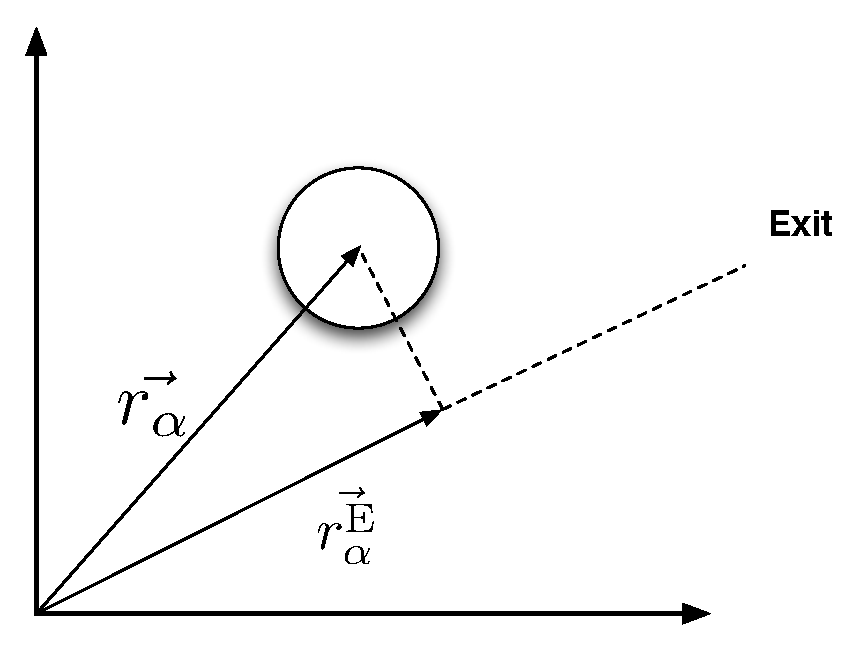
\includegraphics[scale=0.35]{Figures/NotationOfAgent2.pdf}} 
    \caption{Illustration of the vector $ \vec{p_{\alpha}^{E}}$, which is the projection of $ \vec{p_{\alpha}} $ onto the desired direction of motion.}
    \label{impatience}
\end{figure}

\begin{equation}\label{averagespeed}
   \overline{V}_{\alpha} \left( t \right) =
   \frac{1}{t} \overrightarrow{p_{\alpha}}\cdot \overrightarrow{e_{\alpha}} 
\end{equation}

$\overline{V}_{\alpha}$ is undefined at $t=0$ beacause that would mean 
that you should devide by zero, which is undefined. This in turn means 
that $\eta_{\alpha}(0)$ is undefined. We therefore define 
$V_{\alpha}^{0}(t)$ for $t=0$ and $t>0$ to be the following:

\begin{equation}\label{eqn:cond-define}
  V_{\alpha}^{0} (t) = \left\{ 
  \begin{array}{l l}
    V_\alpha^0(0) & \text{if $t=0$}\\
    \left[ 1 - \eta_{\alpha} \left( t \right) \right] 
    V_{\alpha}^{0} \left( 0 \right) +
    \eta_{\alpha} \left( t \right)V_{\alpha}^{\text{max}} & \text{if 
    $t > 0$}\\
  \end{array} \right.
\end{equation}
% TODO: This definition is a tautology. We need a different notation for 
% initial desired velocity.

If we look at the expression for $V_{\alpha}^{0}$ for $t>0$ we can 
start to analyse how this affects the behavior of the agent. There 
are three cases that is of interestes, namely $0 < \eta_{\alpha} < 1$, 
$\eta_{\alpha} < 0$ and $1 < \eta_{\alpha} $.

In the case where $0 \leq \eta_{\alpha} \leq 1$ the expression for 
$V_{\alpha}^{0} \left( t \right)$ makes a lot of sense. Here we can see why this term 
is called the impatience of the agent. If the fraction  between the average 
speed in the desired direction and the initial desired speed is low then 
$\eta_{\alpha} \approx 1$. 
When the impatience term is close to one $V_{\alpha}^{0} \left( t \right)$ is 
dominated by $V_{\alpha}^{\text{max}}$. That is, if the agent have not moved 
very far in the desired direction compared to the initial speed the impatience 
of the agent will cause the agent's future velocity to be dominated by the 
maximum desired velocity of the agent. 
If the agent has been moving in the desired direction with his initial speed 
the entire time then $\eta_{\alpha} = 0$  and $V_{\alpha}^{0} \left( t 
\right)$ will continue to be $V_{\alpha}^{0} \left( 0 \right)$. 

However in the case where $\eta_{\alpha} < 0$, that is the agent has moved 
further in the desired direction than he would have had he been walking with his 
initial speed. This can happen in situations where then agent is being pushed 
forward forward by the crowd.

In the case where $1 < \eta_{\alpha}$ that is the agent has moved further 
in the opposite direction than the desired one. Then can happen if the agent 
starts out by being very close to another agent. However this is not something 
that we think will happen very often. In any circumstances it will only have an 
effect very early in the simulation. 

We see that desired force is mainly controlled by the two parameters $V_{\alpha}^{0} (0)$, 
$V_{\alpha}^{\text{max}}$ and $\overline{V_{\alpha}}$.

This concludes the explanation of the first of the four physical forces. The next 
force in the equation is the repulsive force from the walls.

\begin{center}
\begin{tabular}{lll}
\hline
$\overrightarrow{V_{\alpha}}$ & The actual velocity of agent alpha &\\
\hline
$V_{\alpha}^{0}(t)$ & The desired speed of agent alpha &\\
\hline
$V_{\alpha}^{0}(0)$ & The initial desired speed of agent alpha &\\
\hline
$\overline{V_{\alpha}(t)}$ & The average speed of agent alpha &\\
\hline
$\overrightarrow{p_{\alpha}}$ & The position vector of agent alpha\\
\hline
$e_{\alpha}$& The desired direction of agent alpha\\
\hline
$\tau$& The relaxation time &\\
\hline
\end{tabular}
\end{center}

\subsection{Repulsion from the walls}
The second term on the right hand side of equation \eqref{model} is a force which 
arise from interactions with the walls or other obstacles. It is given by:

\begin{equation}\label{wallpotential}
    \overrightarrow{f_{\alpha B}} \left( \overrightarrow{p_{\alpha}} \right) =
    - \nabla_{\overrightarrow{p_{\alpha}}} U_{B}
    \left( \| \overrightarrow{p_{\alpha}} - \overrightarrow{p_{B}^{\alpha}} \| \right)
\end{equation}

$U_B$ is a repulsive potential and $\|\overrightarrow{p_{\alpha}} - \overrightarrow{p_{B}^{\alpha}}\|$ 
is the distance from the position of agent $\alpha$ to the nearest point on the 
wall as shown in figure \ref{NotationOfWall}. Since $U_B$ is a function of the distance 
$\| \overrightarrow{p_{\alpha}} - \overrightarrow{p_{B}^{\alpha}} \|$, the gradient of $U_B$ tells us in 
which direction this repulsion change the most. It is obvious that the change is 
largest if the agent takes a step directly towards or away from the point in the wall, 
which means that the agent will be pushed directly away from the point in the wall.

\begin{figure}[ht]
\centering
{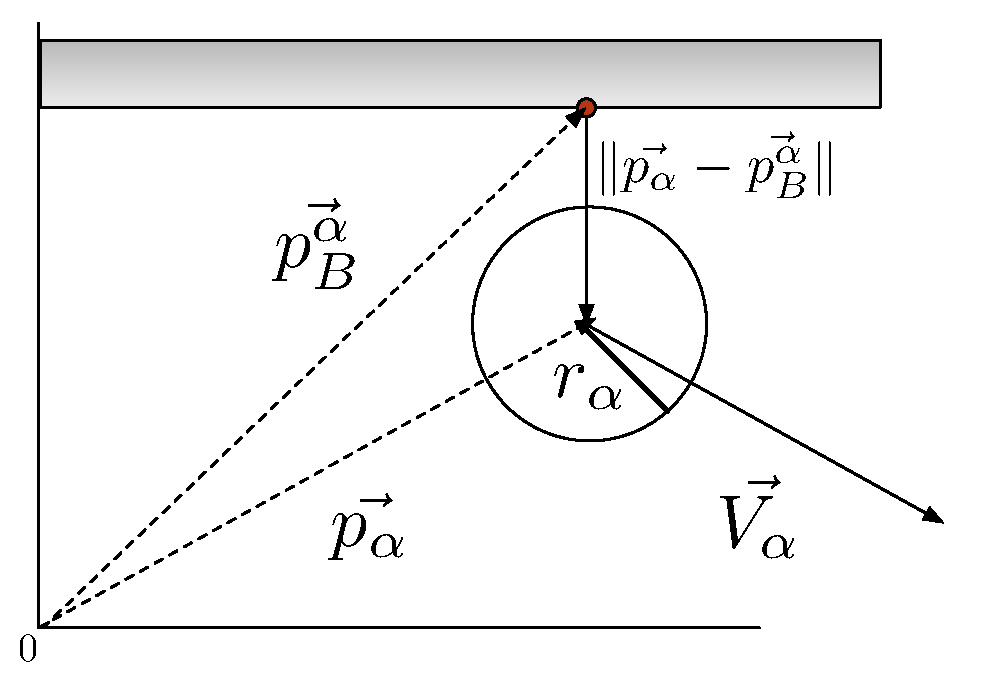
\includegraphics[scale=0.35]{Figures/NotationOfWall.pdf}} 
\caption[Notation of the interaction between an agent and a wall]{The illustration shows the mathematical notation for the interaction with walls used. The circle is pedestrian $\alpha$ with radius $R_{\alpha}$, $\overrightarrow{p_{\alpha}}$ is the position vector for $\alpha$, the grey box on the top is the wall, $\overrightarrow{p_{B}^{\alpha}}$ is the position vector for the closest part of the wall to $\alpha$, $\left( \| \overrightarrow{p_{\alpha}} - \overrightarrow{p_{B}^{\alpha}} \| \right)$ is the smallest distance from $\alpha$ to the wall and $\overrightarrow{V_{\alpha}}$ is the velocity vector for $\alpha$.}
\label{NotationOfWall}
\end{figure}

In order to do the actual calculation we need to know the explicit expression for 
$ \| \overrightarrow{p_{\alpha}} - \overrightarrow{p_{B}^{\alpha}} \|$. First we need to find point on the wall 
that is perpendicular to $\alpha$ as this will be the nearest point to $\alpha$. If we define 
the wall as a vector, $\overrightarrow{W}$ going from a point in space $w_1$ to another point $w_2$, then 
we can find the projection of $\alpha$'s position onto the wall and this projection will be 
$\overrightarrow{p_{B}^{\alpha}}$. This projection is given by:

\begin{equation}\label{wall}
\overrightarrow{p_{B}^{\alpha}}=\frac{\overrightarrow{p_{\alpha}}\cdot \overrightarrow{W}}{\| \overrightarrow{W} \|^2}\overrightarrow{W}
\end{equation}

With this we now have the two points we need to calculate $\|\overrightarrow{p_{\alpha}} - \overrightarrow{p_{B}^{\alpha}}\|$ 
since the position of $\alpha$ is know at all times.

With the explicit expression for $ \| \overrightarrow{p_{\alpha}} - \overrightarrow{p_{B}^{\alpha}} \| $ 
in hand we are able to calculate $\overrightarrow{f_{\alpha B}} \left( \overrightarrow{p_{\alpha}} \right)$ from 
Equation \ref{wallpotential}, as long as the expression for the potential function 
$U_{B}\left( \| \overrightarrow{p_{\alpha}} - \overrightarrow{p_{B}^{\alpha}} \| \right)$ is given. This is 
however not the case in the main article we are working with. In another articles \cite{ABconstant} by 
the same author the repulsive potential from the wall is given by: 

\begin{equation}
U_{B} \left( \| \overrightarrow{p_{\alpha}} - \overrightarrow{p_{B}^{\alpha}} \| \right) =
U^0_{\alpha B} e^{- \| \overrightarrow{p_{\alpha}} - \overrightarrow{p_{B}^{\alpha}} \| / R_{\alpha} }
\end{equation}

where $U^0_{\alpha B}$ is a constant and $R_{\alpha}$ is the radius of a pedestrian $\alpha$.
In that case, the repulsive force on agent $ \alpha $ from the wall is:

\begin{equation}
    \overrightarrow{f_{\alpha B}} \left( \overrightarrow{p_{\alpha}} \right) =
    - \nabla_{\overrightarrow{p_{\alpha}}} U_{B}
    \left( \| \overrightarrow{p_{\alpha}} - \overrightarrow{p_{B}^{\alpha}} \| \right)\\
=-\left( \frac{\partial}{\partial x_{\alpha}}U_{B}( \| \overrightarrow{p_{\alpha}} - \overrightarrow{p_{B}^{\alpha}} \|), \frac{\partial}{\partial y_{\alpha}}U_{B}( \| \overrightarrow{p_{\alpha}} - \overrightarrow{p_{B}^{\alpha}} \|)\right)
\end{equation}

Calculating the derivatives we use that
$\| \overrightarrow{p_{\alpha}} - \overrightarrow{p_{B}^{\alpha}} \|= \sqrt{(x_{\alpha}-x^{\alpha}_{B})^2+(y_{\alpha}-y^{\alpha}_B)^2}$.
Inserting this and the expression for $U_{B}$ we get:

\begin{equation}
\begin{split}
\overrightarrow{f_{\alpha B}} \left( \overrightarrow{p_{\alpha}} \right) 
& =-\left( \frac{\partial}{\partial x_{\alpha}}U^0_{\alpha B} e^{-\sqrt{(x_{\alpha}-x^{\alpha}_{B})^2+(y_{\alpha}-y^{\alpha}_B)^2}/R_{\alpha} }\right. , \\
& \left. \frac{\partial}{\partial y_{\alpha}}U^0_{\alpha B} e^{-\sqrt{(x_{\alpha}-x^{\alpha}_{B})^2+(y_{\alpha}-y^{\alpha}_B)^2}/R_{\alpha} } \right)
\end{split}
\end{equation}

The differentiation then gives: 

\begin{equation}\label{eqn:wall-repulsion}
    \overrightarrow{f_{\alpha B}} \left( \overrightarrow{p_{\alpha}} \right) 
=-\left(U^0_{\alpha B}\frac{1}{R_{\alpha}}\frac{e^{- \| \overrightarrow{p_{\alpha}} - \overrightarrow{p_{B}^{\alpha}} \| / R_{\alpha} } (x_{\alpha}-x_B^{\alpha})}{\| \overrightarrow{p_{\alpha}} - \overrightarrow{p_{B}^{\alpha}} \| },U^0_{\alpha B}\frac{1}{R_{\alpha}}\frac{e^{- \| \overrightarrow{p_{\alpha}} - \overrightarrow{p_{B}^{\alpha}} \| / R_{\alpha} } (y_{\alpha}-y_B^{\alpha})}{\| \overrightarrow{p_{\alpha}} - \overrightarrow{p_{B}^{\alpha}} \| }\right) \\
\end{equation}

The exponential function will always lay between 0 and  1:

\begin{equation}
0 < e^{ -\| \overrightarrow{p_{\alpha}} - \overrightarrow{p_{B}^{\alpha}} \| /R_\alpha} < 1
\end{equation}

Which leads to:

\begin{equation}
0< U_{B} \left( \| \overrightarrow{p_{\alpha}} - \overrightarrow{p_{B}^{\alpha}} \| \right) < U^0_{\alpha B}
\end{equation}

We can see that this force act in the following way: $\overrightarrow{f_{\alpha B}}$ tends to 0 as the distance 
$\| \overrightarrow{p_{\alpha}} - \overrightarrow{p_{B}^{\alpha}} \|$ gets large, meaning that a pedestrian in a reasonably 
distance from the wall will feel a diminishing force. $\overrightarrow{f_{\alpha B}}$ tends to $U^0_{\alpha B}$ 
as the distance $ \| \overrightarrow{p_{\alpha}} - \overrightarrow{p_{B}^{\alpha}} \|$ tends to $0$ the pedestrian will be 
pushed, with some force depending on $U^0_{\alpha B}$, away from the wall. The negative of the force 
means that when the potential between wall and pedestrian rises so will the force, but in the opposite 
direction meaning that the pedestrian will be pushed away. This can be understood as if the pedestrian 
is trying to avoid the wall as it is expected from real life situations. \cite{social-force}. %real references, please.

\begin{center}
\begin{tabular}{lll}
\hline
$\overrightarrow{p_{\alpha}^{\text{B}}}$& Vector pointing from origo to the point on the wall nearest to agent alpha &\\
\hline
$\overrightarrow{W}$& Vector representing the wall &\\
\hline
$U_{B}$ & Repulsive potential from the wall\\
\hline
$U^{0}_{\alpha B}$ & Constant representing agent alpha's tendency to avoid walls\\
\hline
$R_{\alpha}$& Repulsive potential from the wall\\
\hline
\end{tabular}
\end{center}

\subsection{Repulsion from other agents}
The third term on the right hand side of equation \eqref{model} is a summation of all the 
force between agent $\alpha$ and agent $\beta$. The equation we use is taken from a newer article \cite{ABconstant}. We did this because the original article contains two constants that is not given in the articel and in a mail we were adviced, by the authors, to use the values and equation from the new article. 

The function for the repulsion between pedestrians depends on the position vector and the velocity of 
both agents, and it is given by:

\begin{equation}
        \overrightarrow{f_{\alpha \beta }}\left( t \right) = w\left(\phi_{\alpha \beta}\right)\overrightarrow{g}\left(d_{\alpha \beta}(t)\right)
    \label{eq:agentinteraction}
\end{equation}

The two functions that gives the repulsion between the pedestrians is respectively the angel dependece, $ w\left(\phi_{\alpha \beta}\right)$, and the pure force without any angle dependence, $\overrightarrow{g}\left(d_{\alpha \beta}(t)\right)$.

$ w\left(\phi_{\alpha \beta}\right)$ is given as: 

\begin{equation}
    w\left(\phi_{\alpha \beta}\right)=
    \left(
        \lambda_{\alpha} + \left(
            1 - \lambda_{\alpha}
        \right)
		\frac{1+\cos{\phi}}{2}
    \right) 
    \label{angleAB}
\end{equation}

the angle $\phi_{\alpha \beta}$ is the angle between the 
vector pointing from agent $\beta$ to $\alpha$ and the direction in which 
agent $\alpha$ is moving. Cosine to the angle is 

\begin{equation}
\cos \left( \phi \left( t \right) \right)
		= 
	- \overrightarrow{\eta_{\alpha \beta}}
		\left( t \right) 
	\cdot 
\overrightarrow{e_{\alpha}}\left( t \right)
\end{equation}

$\lambda_{\alpha}$ is governing a persons tendency to focus on things happening in front of him 
rather than behind him. It will have a value  $0\leq \lambda_{\alpha}\leq 1$

A value of $\lambda_{\alpha}=1$ means that the force won't depent on the angle. Thus $\alpha$ will react the same to $\beta$ no matter if $\beta$ is in the front or comes from the side or back. A value of $0$ will on the other hand give the maximum angle depence. We find that $0\leq w\left(\phi_{\alpha \beta}\right)\leq1$ when $-1 \leq \cos \left( \phi \right) \left( t \right) \leq 1$. From this we see that $\alpha$ wont be affected at all if $\beta$ is coming from behind and the force will be maximum when $\beta$ comes directly in the front. It should be noted that in general one will find that the maximum of $w\left(\phi_{\alpha \beta}\right)$ always will be $1$ and the minimum will be equal to $\lambda_{\alpha}$.   

% we should make a drawing of this.

The force, without the effect of $w\left(\phi_{\alpha \beta}\right)$, is given as the second term, in the right hand side of equation \ref{eq:agentinteraction}. The function is:  

\begin{equation}
	\overrightarrow{g} 
	\left(
	d_{\alpha \beta}
	\right)
	=
	 A_{\alpha} e^{ \left(\frac{ R_{\alpha \beta} - d_{\alpha \beta}}{B_{\alpha}}\right)}
	\overrightarrow{n}_{\alpha \beta}
	        \label{re}	
\end{equation}

Here $A_{\alpha}$ and $B_{\alpha}$ are constants that can differ for each agent. 
$R_{\alpha \beta}$ is the sum of the radii of $\alpha$ and $\beta$ that is 
$R_{\alpha \beta} = R_{\alpha} + R_{\beta}$. $d_{\alpha \beta}$ is the 
distance from the center of agent $\alpha$ and the center of 
agent $\beta$ and is therefore given by $d_{\alpha \beta} = 
\|\overrightarrow{p_{\alpha}}\left( t \right) - \overrightarrow{p_{\beta}}\left( t \right) \|$.
$\eta_{\alpha \beta}$ is the unit vector pointing from $\alpha$ to $\beta$ 
and it is given by:

\begin{equation}
    \eta_{\alpha \beta} =
        \frac{\overrightarrow{p_{\alpha}}(t) - \overrightarrow{p_{\beta}}(t)}
             {\|\overrightarrow{p_{\alpha}}(t) - \overrightarrow{p_{\beta}}(t) \|}
\end{equation}

\begin{figure}[ht]
    \centering
    {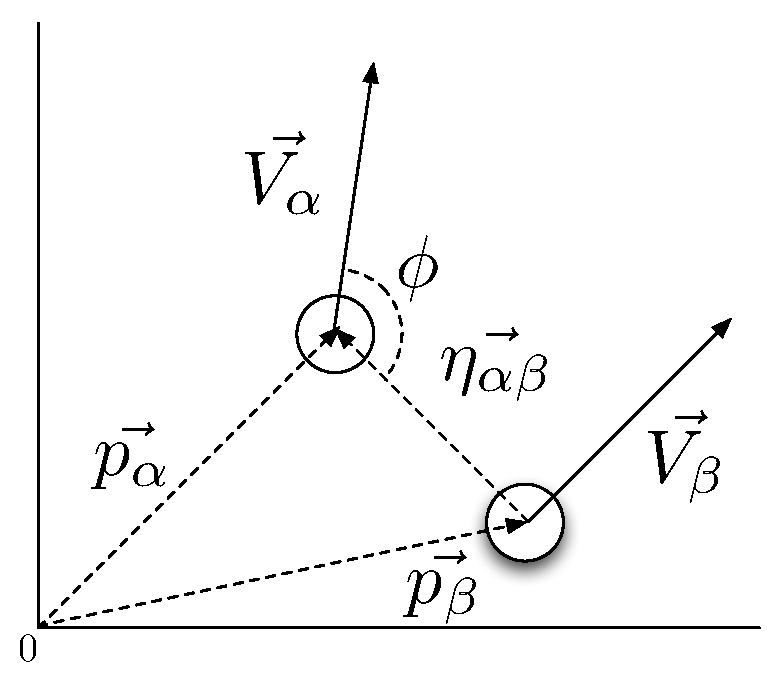
\includegraphics[scale=0.35]{Figures/NotationOfInteraction.pdf}} 
    \caption[Notation of the interaction between two agents]{Illustration of the notation for the interaction between agents.
	     An addition and difference to \ref{NotationOfWall} is that the wall has been replaced by pedestrian $\beta$.
	     $\eta_{\alpha \beta}$ is the vector pointing from $\alpha$ to $\beta$, and $\phi$ is the angle between $\alpha$'s 
	     velocity vector and the vector to $\beta$.}
    \label{fig:NotationOfInteraction}
\end{figure}


%Equation \ref{agentinteraction} is given by two terms. 
%The first term determines how much the the angle between the agents is and how much this angle should affect the force. 
%The constant $\lambda$ is the one controling the importance of the angle.
%The second term reflects the pedestrians tendency to stay at a certain distance 
%from other agents. The constants $A_{\alpha}$, $B_{\alpha}$ is the strength 
%and range of the interaction respectively and controls how big the force will be at a certain distance.  

Taking the norms of both sides of Equation (\ref{re}), we can draw the relation between the value of $\overrightarrow{f_{\alpha\beta}}(t)$ and $ d_{\alpha\beta} $, as shown in Figure 
(\ref{fig:physicalinteraction2}).\\

\begin{figure}[hb]
    \centering
    {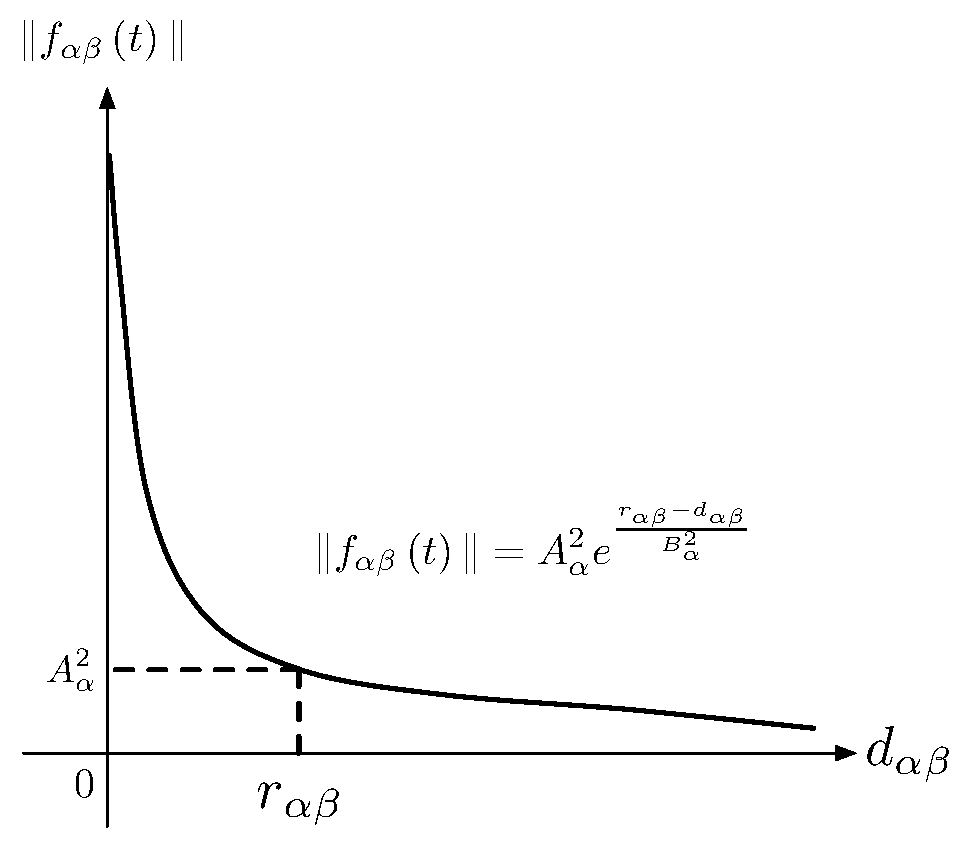
\includegraphics[scale=0.45]{Figures/physicalinteraction.pdf}} 
    \caption[Psysical interaction]{Illustration of the function about the interaction force 
        $f_{\alpha\beta}(t)$ and the distance between two agents
        $d_{\alpha \beta}$. It follows that the smaller the distance between two agents, the greater the interaction force is. }
    \label{fig:physicalinteraction2}
\end{figure}

There is one intersection of the graph and the  axis at:

\begin{equation}
	\left( d_{\alpha \beta} , \| \overrightarrow{f_{\alpha \beta}} \left( t \right) \| \right)
 =
	\left( 0 , A_{\alpha} exp\left( \frac{R_{\alpha\beta} }{B_{\alpha}}\right)  \right) 
\end{equation}

If we put in values for the constants, we will be able to get a maximum value of $ f_{\alpha\beta}(t) $, 
since the distance between agents cannot be negative. Here we take values from \cite{ABconstant} $ A_{\alpha} = 0.42 m/s^{2} $, 
$ R_{\alpha\beta} = 0.6 m $, and $ B_{\alpha} = 1.65 m $, so 
$ f_{\alpha\beta}(t)^{max} < 0.64 m/s^{2} $. It can never be exactly $0.64m/s^2$ since the vector between $\alpha$ and $\beta$ will be undefined when two pedestrians are in the exact same spot.

%TODO: remember to finish this section
%TODO: again lets  have a little summation here. What kinds of dynamics does the
% social interaction part of the model yield.

\begin{center}
\begin{tabular}{lll}
\hline
$d_{\alpha \beta}$& The distance from agent $\alpha$ to $\beta$ &\\
\hline
$R_{\alpha\beta}$& The sum of the radii of agent $\alpha$ and $\beta$ \\
\hline
$\lambda_{\alpha}$& Anisotropy parameter &\\
\hline
$\eta_{\alpha \beta}$& Normal vector pointing from $\beta$ to $\alpha$ \\
\hline
$A_{\alpha}$& Parameter controlling the interaction streanght \\
\hline
$B_{\alpha}$& Parameter controlling the range of the repulsive interaction  \\
\hline
\end{tabular}
\end{center}

\subsection{The attractive forces between some agents}
The fourth and last term in \eqref{model} represents the force from attraction 
in the room. Attractions can be either be either interesting sculptures, 
sights or familiar persons the agent prefer to be close to, such as friends 
and family. The mathematical structure of this force is the same as the force 
from other agents, however it is opposite in algebraic sign and has different 
constants. 

\begin{figure}[hb] %with some more comments i think that this figure could serve as a summation of the entire section
    \centering
    {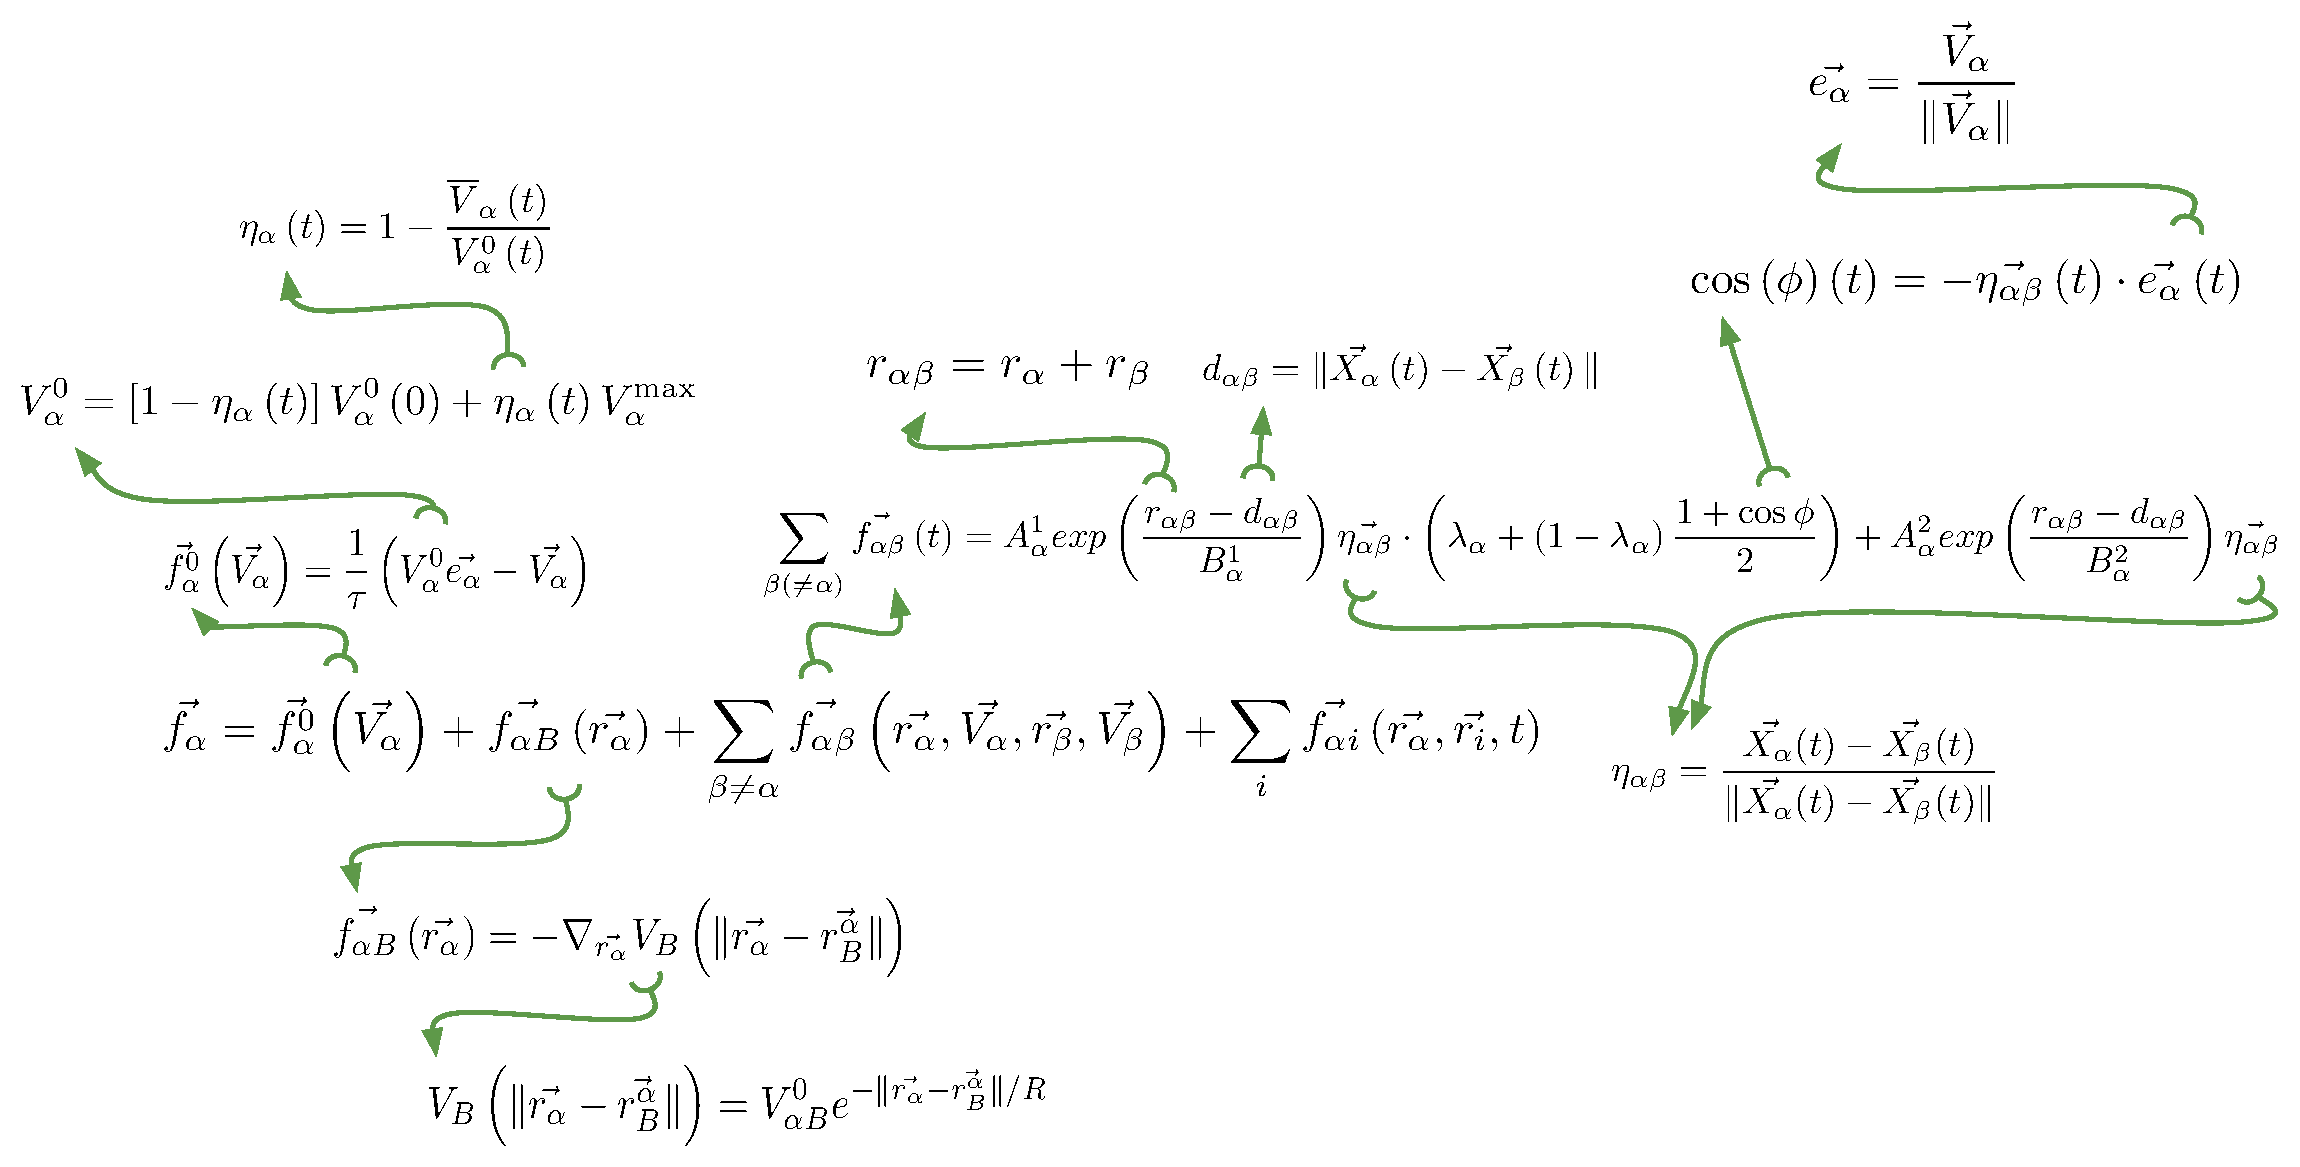
\includegraphics[scale=0.35]{Figures/overview.pdf}} 
    \caption[Overview of the model]{Illustration of an overview of how the model is put together. The different equations and their notation is written to give the 
	     reader an overview of how the model looks like.}
    \label{overview}
\end{figure}

\begin{center}
\begin{tabular}{lll}
\hline
$\overrightarrow{f_{\alpha}^{0}}$ & the desired force &\\
\hline
$\overrightarrow{f_{\alpha B}}$ & the repulsive force from walls &\\
\hline
$\overrightarrow{f_{\alpha \beta}}$ & the repulsion from other agents\\
\hline
$\overrightarrow{f_{\alpha i}}$& the attractive force\\
\hline
$\overrightarrow{V_{\alpha}}$ & The actual velocity of agent alpha &\\
\hline
$V_{\alpha}^{0}(t)$ & The desired speed of agent alpha &\\
\hline
$V_{\alpha}^{0}(0)$ & The initial desired speed of agent alpha &\\
\hline
$\overline{V_{\alpha}(t)}$ & The average speed of agent alpha &\\
\hline
$\overrightarrow{p_{\alpha}}$ & The position vector of agent alpha\\
\hline
$e_{\alpha}$& The desired direction of agent alpha\\
\hline
$\tau$& The relaxation time &\\
\hline
$\overrightarrow{p_{\alpha}^{\text{B}}}$& Vector pointing from origo to the point on the wall nearest to agent alpha &\\
\hline
$\overrightarrow{W}$& Vector representing the wall &\\
\hline
$U_{B}$ & Repulsive potential from the wall\\
\hline
$U^{0}_{\alpha B}$ & Constant representing agent alpha's tendency to avoid walls\\
\hline
$R_{\alpha}$& Repulsive potential from the wall\\
\hline
$d_{\alpha \beta}$& The distance from agent $\alpha$ to $\beta$ &\\
\hline
$R_{\alpha\beta}$& The sum of the radii of agent $\alpha$ and $\beta$ \\
\hline
$\lambda_{\alpha}$& Anisotropy parameter &\\
\hline
$\eta_{\alpha \beta}$& Normal vector pointing from $\beta$ to $\alpha$ \\
\hline
$A_{\alpha}$& Parameter controlling the interaction streanght \\
\hline
$B_{\alpha}$& Parameter controlling the range of the repulsive interaction  \\
\hline
$d_{\alpha \beta}$& The distance from agent $\alpha$ to $\beta$ &\\
\hline
$R_{\alpha\beta}$& The sum of the radii of agent $\alpha$ and $\beta$ \\
\hline
$\lambda_{\alpha}$& Anisotropy parameter &\\
\hline
$\eta_{\alpha \beta}$& Normal vector pointing from $\beta$ to $\alpha$ \\
\hline
$A_{\alpha}$& Parameter controlling the interaction streanght \\
\hline
$B_{\alpha}$& Parameter controlling the range of the repulsive interaction  \\
\hline
\end{tabular}
\end{center}

We have now seen the explicit mathematical expression for the social forces 
as well as explained how this affects the behavior of the agents. To get an 
overview of how the model is put together look a figure \ref{overview} with 
the aid of table. In section \ref{sec:assessment} 
we discuss some of the models features in more detail as well as some features 
that the model does not have. For the implementation of the model see section \ref{sec:simulation}.
